\documentclass[
	%parspace, % Térköz bekezdések közé / Add vertical space between paragraphs
	%noindent, % Bekezdésének első sora ne legyen behúzva / No indentation of first lines in each paragraph
	nohyp, % Szavak sorvégi elválasztásának tiltása / No hyphenation of words
	%twoside, % Kétoldalas nyomtatás / Double sided format
	%final, % Teendők elrejtése / Set final to hide todos
]{elteikthesis}[2021/05/15]

% Dolgozat metaadatai
\title{Időpont foglaló webes alkalmazás} % cím / title
\date{2021} % védés éve / year of defense

% Szerző metaadatai
\author{Andi Péter}
\degree{programtervező informatikus BSc}

% Témavezető(k) metaadatai
\supervisor{Dr. Menyhárt László Gábor} % belső témavezető neve / internal supervisor's name
\affiliation{adjunktus} % belső témavezető beosztása / internal supervisor's affiliation
%\extsupervisor{Külső Kornél} % külső témavezető neve / external supervisor's name
%\extaffiliation{informatikai igazgató} % külső témavezető beosztása / external supervisor's affiliation

% Egyetem metaadatai
\university{Eötvös Loránd Tudományegyetem} % egyetem neve / university's name
\faculty{Informatikai Kar} % kar neve / faculty's name
\department{Média- és Oktatásinformatikai\\ Tanszék} % tanszék neve / department's name
\city{Budapest} % város / city
\logo{elte_cimer_szines} % logo

% Irodalomjegyzék hozzáadása
\addbibresource{thesis.bib}

% A dolgozat
\begin{document}

% Nyelv kiválasztása
\documentlang{magyar}
%\documentlang{english}

% Teendők listája (final dokumentumban nincs)
\listoftodos[\todolabel]

% Dokumentum beállítások
% Lábjegyzet folytonos számozása fejezetek között
% Continuous counting of footnotes among chapters
\counterwithout{footnote}{chapter}

% Tartalomjegyzék oldalszámozásának rejtése
% Hide page numbering of ToC
\newcounter{conpageno}
\let\oldtableofcontents\tableofcontents
\renewcommand{\tableofcontents}{
	\pagenumbering{gobble}
	\oldtableofcontents
	\cleardoublepage
	\setcounter{conpageno}{\value{page}}
	\pagenumbering{arabic}
	\setcounter{page}{\value{conpageno}}
}


% Címlap (kötelező)
\todo{Milyen tanszék?}
\maketitle

\topicdeclaration

% Tartalomjegyzék (kötelező)
\tableofcontents
\cleardoublepage

% Tartalom
\chapter{Bevezetés}
\label{ch:intro}

\section{Motiváció}
Szakdolgozatom célja egy időpont foglaló webes alkalmazás létrehozása. A motivációt unokatestvérem adta, aki személyi edzőként dolgozik. A munkájához elengedhetetlen, hogy időpontot egyeztessen ügyfeleivel. Ezt üzenetváltásokkal tette, viszont, ha valaki lemondott egy időpontot, akkor utána arra a szabad időpontra más ügyfelet körülményes volt találni a platform miatt. Arról nem is beszélve, hogy hónap végén a számlakiállításhoz így nem volt egy konkrét listája, amit egyszerűen be tudott volna vinni a számlázó rendszerébe.

Én programozásban mindig is webes alkalmazások fejlesztését élveztem a legjobban, így amikor felvetette az ötletet, hogy lehetne egy időpont foglaló alkalmazást csinálni, le is csaptam rá. Ezzel nem csak az egész eddigi összes webes tudásomat tesztelhetem és fejleszthetem, hanem segíthetek is unokatestvéremnek, aki nagyon sokat segített rajtam is.

\section{Megvalósítandó alkalmazás leírása}
Az alkalmazásnak két fő felhasználói köre van, a vállalkozók és az ügyfelek.

Az ügyfelek tudnak a vállalkozók között böngészni, egyes vállalkozók időpontjait megnézni, szűrni és lefoglalni. Megnézhetik a lefoglalt időpontjaikat, melyeket lemondhatnak.

A vállalkozók létrehozhatnak kategóriákat (pl.: személyi edzés, angol korrepetálás), melynek megadhatnak árat, maximum résztvevő számot és hogy publikus-e az esemény, vagy csak megadott ügyfelek láthatják. Ez azért fontos, mert például unokatestvérem hétvégére csak családtagoknak vagy közeli ismerősöknek tartott edzéseket, az alkalmazásban ezért kell tudni szabályozni a láthatóságát a kategóriáknak. A vállalkozók időpont hirdetésnél választhatnak egy kategóriát és kezdő és vég időpontot, esetleg módosíthatják a résztvevő limitet. A kategóriákat, időpontokat és vállalkozói profilt lehet szerkeszteni. A vállalkozó le tudja kérdezni, kategóriákra és időtartamra szűrhetően, hogy egy ügyfél melyik kategóriából hány időpontot foglalt, ezek mennyibe kerültek összesen és generálhat egy pdf formátumú számlát.

\section{Kedvhozó az architektúrához}
A dolgozatomban nem csak a programra koncentráltam, hanem, hogy a mögöttes architektúra és kód minőségi és bővíthető legyen.

A backendem Uncle Bob Clean Architecture\cite{cleanArchitecturePost} elvén alapuló objektum orientált kód. Ezzel moduláris, elkülönített hatáskörű osztályokból áll a REST API-om, mellyel a Dependency Inversion Principle miatt egyszerűen és hatékonyan unit- és integrációs tesztelhető az alkalmazás.

A frontendemen React.js-t\footnote{React.js - \href{https://reactjs.org/}{https://reactjs.org/}} használok Typescript-el, e miatt erős fordítási idejű garanciát kapok, hogy a kódom helyes. Továbbá a Typescript erős típusrendszere miatt a megjelenítés mögött funkcionális paradigmájú kód van. Ez azt jelenti, hogy nincs destruktív értékadás, összeg típusokkal és egy saját aszinkron Result monád típus miatt nem kivételeket kezelek, hanem típus szintű konstrukciókkal garantálom, hogy minden hiba megfelelően le legyen kezelve és programozói hibából ne lehessen inkonzisztens állapotban levő adathoz hozzáférni.

\cleardoublepage

\chapter{Felhasználói dokumentáció} % User guide
\label{ch:user}

\section{Rendszerkövetelmények}
Szerver oldalon: Windows 10 vagy Linux operációs rendszer, 2GB RAM, legalább 5GB tárhely az adatoknak, port nyitási lehetőség.

\todo{Telefonra ha meg lesz akkor az jöhet ide}
Kliens oldalon: Legalább Chrome 90, Firefox 88, Edge 90, ezek mind asztali számítógépen, legalább 1280x720-as képernyő felbontással.

\section{Telepítés}

Az alkalmazást legegyszerűbben Docker\footnote{\url{https://www.docker.com/}} segítségével lehet telepíteni. Van lehetőség Docker nélkül is, viszont az több konfigurációval és üzemeltetéssel jár.

\subsection{Telepítés Dockerrel}

A Dockeres telepítéshez szükséges a Docker\footnote{\url{https://www.docker.com/get-started}} és Docker Compose\footnote{\url{https://docs.docker.com/compose/install/}} telepítése.

A fő mappában megtalálható \textit{docker-compse.yml} fájlban találhatók meg a konténerek konfigurációi. Három konténerből áll, egy MariaDB \footnote{\url{https://mariadb.org/}} adatbázisból, a backend REST API-ból és a frontendből.
A yml fájlban a következő konfigurációs lehetőségek a \ref{tab:config} táblázatban találhatók.

Az alap beállításokkal a \textit{http://localhost:8100}-on érhető el az alkalmazás. HTTPS-t, tűzfalat érdemes bekonfigurálni egy Reverse Proxy\cite{nginxReverseProxy}-val, például Nginx-el.

\todo{Content elrendezése nagy page break nélkül}
\begin{table}[H]
	\centering
	\begin{tabular}{ | m{0.25\textwidth} | m{0.25\textwidth} | m{0.45\textwidth} | }
		\hline
		\textbf{Konfigurációs változó} & \textbf{Alap érték} & \textbf{Megjegyzés} \\
		\hline \hline
		\multicolumn{3}{|l|}{db} \\
		\hline
		\tiny{MYSQL\_ROOT\_PASSWORD} & kebab & MariaDB adatbázis root felhasználójának jelszava \\
		\hline
		\small{volumes} & \tiny{./db\_data:/var/lib/mysql} & MariaDB adatbázis perzisztens tárolása a lokális db\_data mappában  \\ \hline
		\small{ports} & 3306:3306 & A konténer 3306-as portja a hoston az 3306-es portra forwardolása \\ \hline
		\hline \hline
		\multicolumn{3}{|l|}{backend} \\
		\hline
		\small{IWA\_CorsAllowUrls} & http://127.0.0.1:8100 & Vesszővel elválasztva az engedélyezett publikus frontend url-ek. Pl.: \url{https://andipeter.me} \\ \hline
		\small{IWA\_MYSQL\_HOST} & db & MariaDB adatbázis host neve \\ \hline
		\small{IWA\_MYSQL\_PORT} & 3306 & MariaDB adatbázis portja \\ \hline
		\small{IWA\_MYSQL\_DB} & iwa & MariaDB adatbázison belül használandó adatbázis \\ \hline
		\small{IWA\_MYSQL\_USER} & root & MariaDB adatbázis felhasználója \\ \hline
		\small{IWA\_MYSQL\_PASS} & kebab & MariaDB adatbázis felhasználójának jelszava \\ \hline
		\small{volumes} & \tiny{./avatars:/app/AvatarData} & A profilképek perzisztens tárolása a lokális avatars mappában  \\ \hline
		\small{ports} & 5000:80 & A konténer 80-as portja a hoston az 5000-es portra forwardolása \\
		\hline \hline
		\multicolumn{3}{|l|}{frontend} \\
		\hline
		\small{API\_URL} & http://127.0.0.1:5000 & A backend publikus elérési url-je. Pl.: \url{https://andipeter.me}/api/ \\
		\hline
		\small{ports} & 8100:80 & A konténer 80-as portja a hoston az 8100-es portra forwardolása \\ \hline
	\end{tabular}
	\caption{Konfigurációs változók beállításai}
	\label{tab:config}
\end{table}

Az alkalmazást ez után a \textit{docker-compose up} paranccsal indíthatjuk el. Első futtatásra ez eltarthat pár percig, mert a Dockernek le kell töltenie a megfelelő alap konténereket az internetről és utána létre kell hozni ezeket a konténereket a forráskódból.

További docker-compose parancsok a docker-compose dokumentációjábanban\footnote{\url{https://docs.docker.com/compose/reference/}} találhatók.

\subsection{Telepítés Docker nélkül}

Az alkalmazás futtatásához szükség lesz egy MariaDB szerverre és azon belül egy \textit{iwa} nevű adatbázisra. Az alkalmazás Linux és Windows rendszereken is futhat, ehhez a megfelelő backend fájl futtatása szükséges.

A backend futtatása parancssorból az \textit{IWA\_Backend.API} futtatható fájllal lehet. A konfigurációja az \text{appsettings.json} fájlban található, kitöltése a \ref{tab:config} táblázat alapján történik. A backend így a host 80-as portján fog futni. Ezt a \textit{- -urls=http://localhost:5001/} konzoli argumentummal lehet megváltoztatni, ebben az esetben az 5001-es porton futna az alkalmazás.

A frontend statikus HTML, JS és CSS fájlokból áll, ezt például Apache\footnote{\url{https://httpd.apache.org/}} vagy Nginx\footnote{\url{https://www.nginx.com/}} szerverekkel, vagy más hasonló webhost szolgáltatásokkal lehet kitelepíteni. A frontend konfigurációja a mappájában a \textit{config.js} fájlban történik, kitöltési útmutató a \ref{tab:config} táblázatban található.

\section{Funkciók leírása}

Az alkalmazásban lehet regisztrálni ügyfél vagy vállalkozóként. Az oldalt lehet bejelentkezve vagy bejelentkezés nélkül böngészni.

\subsubsection{Kategóriák}

A vállalkozók létrehozhatnak kategóriákat. A kategória effektíve egy időpont típus, például személyi edzés. A kategóriák megegyszerűsítik az új időpontok létrehozását, mert a különböző időpontok közti azonos adatokat enkapszulálják, az időpontnál így csak az időpont specifikus adatokat kell megadni. Egy kategóriának lehet egy leírása, ára, ajánlott max résztvevő száma és láthatósága. Az ajánlott max résztvevőszám azt jelenti, hogy egy új időpont létrehozásánál alapból ez a szám lesz a max résztvevők mezőben, viszont ettől el lehet térni időpontról időpontra, például egy csoportos edzésre a Margit szigeten többen jöhetnek mint a Hősök tereire.

Egy kategória láthatósága a következőt jelenti. Ha nyílt egy esemény, akkor bárki láthatja, bárki jelentkezhet rá. Ha egy esemény nem nyílt, akkor csak azok az emberek láthatják és jelentkezhetnek rá, akik engedélyezett résztvevőként fel lettek véve a kategóriára. Ennek az a szerepe, hogy például egy Családi edzésre hétvégén ne tudjon mindenki jelentkezni, csak az előre felvett családtagok. Vagy például egy kedvezményes árazású időpontnak más lehet a kategóriája.

Kategóriákat nem lehet törölni, abból az okból, hogy akkor az összes hozzá tartozó időpont is törlődne, ezzel múltbeli időpontok adatai elvesznének.

\subsubsection{Időpontok}

Új időpont hirdetésénél az időponthoz kell választani egy kategóriát, kezdő és vég időpontot. Opcionálisan meg lehet változtatni a max résztvevő számot. Van lehetőség alapból felvenni ügyfeleket az időpontra, például ha a vállalkozó már előre leegyeztetett egy időpontot de még nem írta ki az alkalmazáson, akkor az ügyfélnek nem kell bejelentkeznie és lefoglalni az időpontot.

Időpont szerkesztésnél a vállalkozónak van lehetősége változtatni egy időpont összes értékén. A kategórián például azért változtathat, mert Angol óra helyett Német órát tartott az ügyfélnek, vagy Páros edzés helyett Személyi Edzést, mert közbe jött valami. Lehet az időpontra jelentkezett felhasználókat is módosítani, lejelentkeztetni és felvenni ügyfeleket, akár az időpont után is. Például valaki lemondott egy edzést és beugrott helyette valaki más, a nap végén pedig így helyesen tudja adminisztrálni ezt a vállalkozó.

\subsubsection{Számlázás}

A számlázás funkciónál a vállalkozók adott felhasználók lefoglalt időpontjaiból tudnak számlát generálni egy időszakra, például Április 1 és 30 között. Ez a számla jelenlegi formájában nem minősül NAV által elfogadott számlának, viszont a vállalkozónak nagyon jó segítség, hogy a saját számlázó szoftverébe (pl.: számlázz.hu) miről írjon számlát. Az alkalmazásba azért se került online fizetési lehetőség vagy számlázz.hu integráció, mert a valóságban az időpontokon kívül mást is tartalmazni szokott a számla (pl.: edzőterem bérlet, edzésterv) és ezekre akkor ezen felül egy külön számlát kéne kiállítania a vállalkozónak.

\section{Használat}

Regisztráció, bejelentkezés

\subsection{Ügyfeleknek}
Felhasználói leírás, hogy lehet böngészni a vállalkozókat, hogy lehet szűrni az időpontokat, hogy lehet lefoglalni időpontot, foglalt időpontokat hol lehet megnézni, hogy lehet lemondani időpontot, saját profilt megnézni és szerkeszteni

\subsection{Vállalkozóknak}
vállalkozói oldal, kategória létrehozás, szerkesztés, megtekintés

Időpont létrehozás, megtekintés, szerkesztés, törlés

profil szerkesztése, profilkép frissítése

számlázás, szűrés, számla letöltése



















% Lorem ipsum dolor sit amet $\mathbb{N}$\nomenclature{$\mathbb{N}$}{Set of natural numbers}, consectetur adipiscing elit. Duis nibh leo, dapibus in elementum nec, aliquet id sem. Suspendisse potenti. Nullam sit amet consectetur nibh. Donec scelerisque varius turpis at tincidunt. Cras a diam in mauris viverra vehicula. Vivamus mi odio, fermentum vel arcu efficitur, lacinia viverra nibh. Aliquam aliquam ante mi, vel pretium arcu dapibus eu. Nulla finibus ante vel arcu tincidunt, ut consectetur ligula finibus. Mauris mollis lectus sed ipsum bibendum, ac ultrices erat dictum. Suspendisse faucibus euismod lacinia $\mathbb{Z}$\nomenclature{$\mathbb{Z}$}{Set of integer numbers}.


% \section{Felsorolások} % Enumerations and lists

% Etiam vel odio ante. Etiam pulvinar nibh quis massa auctor congue. Pellentesque quis odio vitae sapien molestie vestibulum sit amet et quam. Pellentesque vel dui eget enim hendrerit finibus at sit amet libero. Quisque sollicitudin ultrices enim, nec porta magna imperdiet vitae. Cras condimentum nunc dui, eget molestie nunc accumsan vel.

% \begin{itemize}
% 	\item Fusce in aliquet neque, in pretium sem.
% 	\item Donec tincidunt tellus id lectus pretium fringilla.
% 	\item Nunc faucibus, erat pretium tempus tempor, tortor mi fringilla neque, ac congue ex dui vitae mauris.
% \end{itemize}

% Donec dapibus sodales ante, at scelerisque nunc laoreet sit amet. Mauris porttitor tincidunt neque, vel ullamcorper neque pulvinar et. Integer eu lorem euismod, faucibus lectus sed, accumsan felis. Nunc ornare mi at augue vulputate, eu venenatis magna mollis. Nunc sed posuere dui, et varius nulla. Sed mollis nibh augue, eget scelerisque eros ornare nec.

% \begin{enumerate}
% 	\item\label{step:first} Donec pretium et quam a cursus. Ut sollicitudin tempus urna et mollis.
% 	\item Aliquam et aliquam turpis, sed fermentum mauris. Nulla eget ex diam.
% 	\item Donec eget tellus pharetra, semper neque eget, rutrum diam Step~\ref{step:first}.
% \end{enumerate}

% Praesent porta, metus eget eleifend consequat, eros ligula eleifend ex, a pellentesque mi est vitae urna. Vivamus turpis nunc, iaculis non leo eget, mattis vulputate tellus. Maecenas rutrum eros sem, pharetra interdum nulla porttitor sit amet. In vitae viverra ante. Maecenas sit amet placerat orci, sed tincidunt velit. Vivamus mattis, enim vel suscipit elementum, quam odio venenatis elit\footnote{Phasellus faucibus varius purus, nec tristique enim porta vitae.}, et mollis nulla nunc a risus. Praesent purus magna, tristique sed lacus sit amet, convallis malesuada magna. 

% \begin{description}
% 	\item[Vestibulum venenatis] malesuada enim, ac auctor erat vestibulum et. Phasellus id purus a leo suscipit accumsan.
% 	\item[Orci varius natoque] penatibus et magnis dis parturient montes, nascetur ridiculus mus. Nullam interdum rhoncus nisl, vel pharetra arcu euismod sagittis. Vestibulum ac turpis auctor, viverra turpis at, tempus tellus.
% 	\item[Morbi dignissim] erat ut rutrum aliquet. Nulla eu rutrum urna. Integer non urna at mauris scelerisque rutrum sed non turpis.
% \end{description}

% \subsection{Szoros térközű felsorolások} % Lists with narrow spacing inbetween items

% Phasellus ultricies, sapien sit amet ultricies placerat, velit purus viverra ligula, id consequat ipsum odio imperdiet enim:
% \begin{compactenum}
% 	\item Maecenas eget lobortis leo.
% 	\item Donec eget libero enim.
% 	\item In eu eros a eros lacinia maximus ullamcorper eget augue.
% \end{compactenum}

% \bigskip

% In quis turpis metus. Proin maximus nibh et massa eleifend, a feugiat augue porta. Sed eget est purus. Duis in placerat leo. Donec pharetra eros nec enim convallis:
% \begin{compactitem}
% 	\item Pellentesque odio lacus.
% 	\item Maximus ut nisl auctor.
% 	\item Sagittis vulputate lorem.
% 	\item \todo{Hmm ide kéne még valami}
% \end{compactitem}

% \bigskip

% Vestibulum ante ipsum primis in faucibus orci luctus et ultrices posuere cubilia Curae; Sed lorem libero, dignissim vitae gravida a, ornare vitae est.
% \begin{compactdesc}
% 	\item[Cras maximus] massa commodo pellentesque viverra.
% 	\item[Morbi sit] amet ante risus. Aliquam nec sollicitudin mauris
% 	\item[Ut aliquam rhoncus sapien] luctus viverra arcu iaculis posuere
% \end{compactdesc}


% \section{Képek, ábrák} % Images and figures

% Aliquam vehicula luctus mi a pretium. Nulla quam neque, maximus nec velit in, aliquam mollis tortor. Aliquam erat volutpat. Curabitur vitae laoreet turpis. Integer id diam ligula. Nulla sodales purus id mi consequat, eu venenatis odio pharetra. Cras a arcu quam. Suspendisse augue risus, pulvinar a turpis et, commodo aliquet turpis. Nulla aliquam scelerisque mi eget pharetra. Mauris sed posuere elit, ac lobortis metus. Proin lacinia sit amet diam sed auctor. Nam viverra orci id sapien sollicitudin, a aliquam lacus suscipit, Figure~\ref{fig:example-1}:

% \begin{figure}[H]
% 	\centering
% 	
\includegraphics[width=0.6\textwidth,height=100px]{elte_cimer_szines}
% 	\caption{Quisque ac tincidunt leo}
% 	\label{fig:example-1}
% \end{figure}

% \subsection{Képek szegélyezése} % Framing figures

% Ut aliquet nec neque eget fermentum. Cras volutpat tellus sed placerat elementum. Quisque neque dui, consectetur nec finibus eget, blandit id purus. Nam eget ipsum non nunc placerat interdum.

% \begin{figure}[H]
% 	\centering
% 	
\includegraphics[width=0.6\textwidth,height=100px,frame]{elte_cimer_szines}
% 	\caption{Quisque ac tincidunt leo}
% \end{figure}

% \subsection{Képek csoportosítása} % Subfigures

% In non ipsum fermentum urna feugiat rutrum a at odio. Pellentesque habitant morbi tristique senectus et netus et malesuada fames ac turpis egestas. Nulla tincidunt mattis nisl id suscipit. Sed bibendum ac felis sed volutpat. Nam pharetra nisi nec facilisis faucibus. Aenean tristique nec libero non commodo. Nulla egestas laoreet tempus. Nunc eu aliquet nulla, quis vehicula dui. Proin ac risus sodales, gravida nisi vitae, efficitur neque, Figure~\ref{fig:example-2}:

% \begin{figure}[H]
% 	\centering
% 	\subfigure[Vestibulum quis mattis urna]{
% 		
\includegraphics[width=0.45\linewidth]{elte_cimer_szines}}
% 	\hspace{5pt}
% 	\subfigure[Donec hendrerit quis dui sit amet venenatis]{
% 		
\includegraphics[width=0.45\linewidth]{elte_cimer_szines}}
% 	\caption{Aenean porttitor mi volutpat massa gravida}
% 	\label{fig:example-2}
% \end{figure}

% Nam et nunc eget elit tincidunt sollicitudin. Quisque ligula ipsum, tempor vitae tortor ut, commodo rhoncus diam. Pellentesque habitant morbi tristique senectus et netus et malesuada fames ac turpis egestas. Phasellus vehicula quam dui, eu convallis metus porta ac.


% \section{Táblázatok} % Tables

% Nam magna ex, euismod nec interdum sed, sagittis nec leo. Nam blandit massa bibendum mattis tristique. Phasellus tortor ligula, sodales a consectetur vitae, placerat vitae dolor. Aenean consequat in quam ac mollis. 

% \begin{table}[H]
% 	\centering
% 	\begin{tabular}{ | m{0.25\textwidth} | m{0.65\textwidth} | }
% 		\hline
% 		\textbf{Phasellus tortor} & \textbf{Aenean consequat} \\
% 		\hline \hline
% 		\emph{Sed malesuada} & Aliquam aliquam velit in convallis ultrices. \\
% 		\hline
% 		\emph{Purus sagittis} &  Quisque lobortis eros vitae urna lacinia euismod. \\
% 		\hline
% 		\emph{Pellentesque} & Curabitur ac lacus pellentesque, eleifend sem ut, placerat enim. Ut auctor tempor odio ut dapibus. \\
% 		\hline
% 	\end{tabular}
% 	\caption{Maecenas tincidunt non justo quis accumsan}
% 	\label{tab:example-1}
% \end{table}

% \subsection{Sorok és oszlopok egyesítése} % Multi rows and multi columns

% Mauris a dapibus lectus. Vestibulum commodo nibh ante, ut maximus magna eleifend vel. Integer vehicula elit non lacus lacinia, vitae porttitor dolor ultrices. Vivamus gravida faucibus efficitur. Ut non erat quis arcu vehicula lacinia. Nulla felis mauris, laoreet sed malesuada in, euismod et lacus. Aenean at finibus ipsum. Pellentesque dignissim elit sit amet lacus congue vulputate.

% \begin{table}[htb]
% 	\centering
% 	\begin{tabular}{ | c | r | r | r | r | r | r | }
% 		\hline
% 		\multirow{2}{*}{\textbf{Quisque}} & \multicolumn{2}{ c | }{\textbf{Suspendisse}} & \multicolumn{2}{ c | }{\textbf{Aliquam}} & \multicolumn{2}{ c | }{\textbf{Vivamus}} \\
% 		\cline{2-7}
% 		& Proin & Nunc & Proin & Nunc & Proin & Nunc \\
% 		\hline \hline		
% 		Leo & 2,80 MB & 100\% & 232 KB & 8,09\% & 248 KB & 8,64\% \\
% 		\hline
% 		Vel & 9,60 MB & 100\% & 564 KB & 5,74\% & 292 KB & 2,97\% \\
% 		\hline
% 		Auge & 78,2 MB & 100\% & 52,3 MB & 66,88\% & 3,22 MB & 4,12\% \\
% 		\hline 
% 	\end{tabular}
% 	\caption[Rövid cím a táblázatjegyzékbe]{Vivamus ac arcu fringilla, fermentum neque sed, interdum erat. Mauris bibendum mauris vitae enim mollis, et eleifend turpis aliquet.}
% 	\label{tab:example-2}
% \end{table}

% \subsection{Több oldalra átnyúló táblázatok} % Long tables over multiple pages

% Nunc porta placerat leo, sit amet porttitor dui porta molestie. Aliquam at fermentum mi. Maecenas vitae lorem at leo tincidunt volutpat at nec tortor. Vivamus semper lacus eu diam laoreet congue. Vivamus in ipsum risus. Nulla ullamcorper finibus mauris non aliquet. Vivamus elementum rhoncus ex ut porttitor.

% \begin{center}
% 	\begin{longtable}{ | p{0.3\textwidth} | p{0.7\textwidth} | }
		
% 		\hline
% 		\multicolumn{2}{|c|}{\textbf{Praesent aliquam mauris enim}}
% 		\\ \hline
		
% 		\emph{Suspendisse potenti} & \emph{Lorem ipsum dolor sit amet}
% 		\\ \hline \hline
% 		\endfirsthead % első oldal fejléce
		
% 		\hline
% 		\emph{Suspendisse potenti} & \emph{Lorem ipsum dolor sit amet}
% 		\\ \hline \hline
% 		\endhead % többi oldal fejléce
		
% 		\hline
% 		\endfoot % többi oldal lábléce
		
% 		\endlastfoot % utolsó oldal lábléce
		
% 		\emph{Praesent}
% 		& Nulla ultrices et libero sit amet fringilla. Nunc scelerisque ante tempus sapien placerat convallis.
% 		\\ \hline
		
% 		\emph{Luctus}
% 		& Integer hendrerit erat massa, non hendrerit risus convallis at. Curabitur ultrices, justo in imperdiet condimentum, neque tortor luctus enim, luctus posuere massa erat vitae nibh.
% 		\\ \hline
		
% 		\emph{Egestas}
% 		& Duis fermentum feugiat augue in blandit. Mauris a tempor felis. Pellentesque ultricies tristique dignissim. Pellentesque aliquam semper tristique. Nam nec egestas dolor. Vestibulum id elit quis enim fringilla tempor eu a mauris. Aliquam vitae lacus tellus. Phasellus mauris lectus, aliquam id leo eget, auctor dapibus magna. Fusce lacinia felis ac elit luctus luctus.
% 		\\ \hline
		
% 		\emph{Dignissim}
% 		& Praesent aliquam mauris enim, vestibulum posuere massa facilisis in. Suspendisse potenti. Nam quam purus, rutrum eu augue ut, varius vehicula tellus. Fusce dui diam, aliquet sit amet eros at, sollicitudin facilisis quam. Phasellus tempor metus vel augue gravida pretium. Proin aliquam aliquam blandit. Nulla id tempus mi. Fusce in aliquam tortor.
% 		\\ \hline
		
% 		\emph{Pellentesque}
% 		& Donec felis nibh, imperdiet a arcu non, vehicula gravida nibh. Quisque interdum sapien eu massa commodo, ac elementum felis faucibus.
% 		\\ \hline
		
% 		\emph{Molestie}
% 		& Cras ullamcorper tellus et auctor ultricies. Maecenas tincidunt euismod lectus nec venenatis. Suspendisse potenti. Pellentesque pretium nunc ut euismod cursus. Nam venenatis condimentum quam. Curabitur suscipit efficitur aliquet. Interdum et malesuada fames ac ante ipsum primis in faucibus.
% 		\\ \hline
		
% 		\emph{Vivamus semper}
% 		& In purus purus, faucibus eu libero vulputate, tristique sodales nunc. Nulla ut gravida dolor. Fusce vel pellentesque mi, vel efficitur eros. Nunc vitae elit tellus. Sed vestibulum auctor consequat. 
% 		\\ \hline
		
% 		\emph{Condimentum}
% 		& Nulla scelerisque, leo et facilisis pretium, risus enim cursus turpis, eu suscipit ipsum ipsum in mauris. Praesent eget pulvinar ipsum, suscipit interdum nunc. Nam varius massa ut justo ullamcorper sollicitudin. Vivamus facilisis suscipit neque, eu fermentum risus. Ut at mi mauris.
% 		\\ \hline
		
% 		\caption{Praesent ullamcorper consequat tellus ut eleifend}
% 		\label{tab:example-3}		
% 	\end{longtable}
% \end{center}

\cleardoublepage

\chapter{Fejlesztői dokumentáció} % Developer guide
\label{ch:impl}

\section{Tervezés}

\subsection{Probléma leírása}

\subsection{Felhasználói esetek}
\todo{Ez a kép nem felel meg a margónak, az baj? Legalább átlátható}
A felhasználói esetek a következőképpen néznek ki. A vállalkozó egyben felhasználó is, a felhasználók összes funkcióját tudják használni, ezt nem jelöltem a diagrammban, hogy átlátható maradjon.

\begin{figure}[H]
	\noindent\makebox[\textwidth]{
	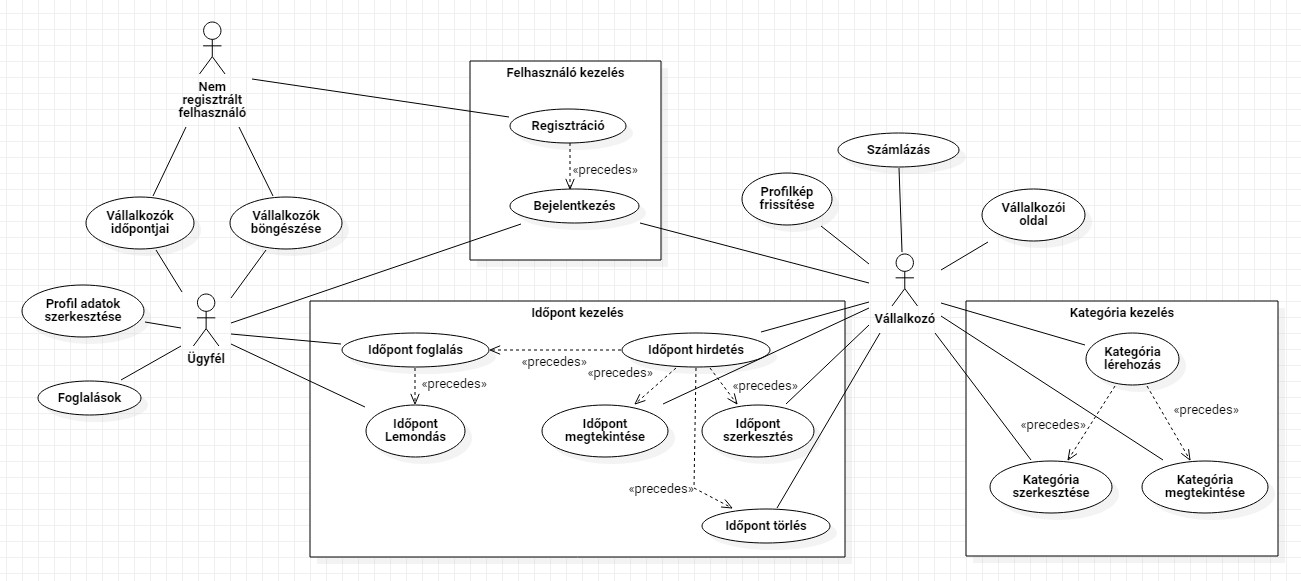
\includegraphics[width=1.3\textwidth]{usecase}}
	\caption{Felhasználói esetek}
	\label{fig:usecases}
\end{figure}

\begin{table}[H]
	\centering
	\begin{tabular}{|l|l|c|}
		\hline
		& \textbf{Leírás} & \textbf{Kód} \\
		\hline
		GIVEN & Nincs bejelentkezve & \multirow{3}{*}{asd} \\ \cline{1-2}
		WHEN & Bejelentkezéshez kötött oldalt nyitna meg & \\ \cline{1-2}
		THEN & Visszairányítódik a főoldalra & \\ 
		\hline
		GIVEN & asd & \multirow{3}{*}{asd} \\ \cline{1-2}
		WHEN & asd & \\ \cline{1-2}
		THEN & asd & \\ 
		\hline
		GIVEN & asd & \multirow{3}{*}{asd} \\ \cline{1-2}
		WHEN & asd & \\ \cline{1-2}
		THEN & asd & \\ 
		\hline
		GIVEN & asd & \multirow{3}{*}{asd} \\ \cline{1-2}
		WHEN & asd & \\ \cline{1-2}
		THEN & asd & \\ 
		\hline
		GIVEN & asd & \multirow{3}{*}{asd} \\ \cline{1-2}
		WHEN & asd & \\ \cline{1-2}
		THEN & asd & \\ 
		\hline
		GIVEN & asd & \multirow{3}{*}{asd} \\ \cline{1-2}
		WHEN & asd & \\ \cline{1-2}
		THEN & asd & \\ 
		\hline
		GIVEN & asd & \multirow{3}{*}{asd} \\ \cline{1-2}
		WHEN & asd & \\ \cline{1-2}
		THEN & asd & \\ 
		\hline
	\end{tabular}
\end{table}

\subsection{REST API vs MVC architektúra}
Webes alkalmazások körében régebben elterjedt volt a Modell-View-Controller architektúra (röviden MVC). Röviden ez azt jelenti, hogy a felhasználó akcióira a Controller réteg eldönti, hogy az állapotot (Modellt) hogy kell frissíteni, ez után pedig egy nézetet (View-t) ad vissza a felhasználónak. A gyakorlatban ez szerver oldali renderelést jelent, például a felhasználó elküld egy űrlapot a szervernek, az feldolgozza és egy szerver által renderelt HTML fájlt küld vissza a felhasználó böngészőjének.

Ennek a megközelítésnek vannak előnyei, többek között, hogy az alkalmazásnak egy kódbázisa van, egyszerűbb egy új funkciót implementálni, kevesebb technológiát is elég ismerni. Hátránya viszont, hogy dinamikus felhasználói felületet nehéz benne építeni, más alkalmazásokba, például mobil alkalmazásba, nem lehet integrálni.

Ezekre nyújt megoldást, ha a logikát egy REST API (Representational state transfer, Application Programming Interface) valósítja meg backenden, a megjelenítésért pedig egy másik program felel frontend-en. A REST egy interfész leíró struktúra, legtöbb esetben HTTP protokoll alapú kommunikációt ír le, melyben JSON formátumú adattal lehet kommunikálni.

Mivel az API-t így programatikusan tudjuk elérni, ezért más alkalmazásokkal egyszerűen képes kommunikálni. Így lehet például web-ről, telefonos- vagy asztali alkalmazásból elérni a biznisz logikát, ezért csak a megjelenítést kell variálni platformok között.

A REST API állapot mentes, ami azt jelenti, hogy a szerver nem függ valamilyen kontextustól, csak a kérésben szereplő adattal elég dolgoznia. Ez lehetővé teszi, hogy a backend több szerveren horizontálisan egy load balancer (terheléselosztó) segítségével legyen skálázva. Egy ilyen rendszerben az egymást követő kérések akár különböző backend példányokhoz futhatnak be, az alkalmazás ugyan olyan pontosan működik.

A programozható felület lehetővé teszi, hogy a szerver ne teljes oldalakat küldjön vissza válasznak, hanem csak adatot. Ez a rugalmasság lehetővé teszi, hogy a frontend dinamikus legyen. Például az én alkalmazásomban egy új időpont hirdetésénél a böngésző tesz egy kérést a szerver felé, ami visszaadja a létrejött időpont adatát és a frontend azt az egy időpontot beilleszti a jelenleg megjelenített időpontok közé, nem kell a teljes oldalt az összes időponttal újra tölteni.

A hátránya ennek az architektúrának, hogy a backend és frontend teljesen különálló, akár más programozási nyelvekben vannak írva, más eszközökkel kell fejleszteni őket, így nagyobb a projekt komplexitása. Vállalati környezetben ez előny lehet, mert külön csapatokra szét lehet osztani a frontend és backend fejlesztést. További nehézség lehet, hogy az backendet és a frontendet össze kell kötni, ez az integráció nem olyan triviális, mint egy monolitikus MVC alkalmazásban, ahol egyből a modell adatát bele lehet renderelni HTML tagek közé. Továbbá, mivel az API így egy külön álló alkalmazás, amit bárhonnan lehet lekérdezni, fontos biztonsági lépésekkel le kell védeni, hogy jogosulatlan adathoz ne lehessen hozzáférni, szennyezett adattal ne lehessen elrontani az alkalmazást.

\subsection{Clean Architecture Backenden}
\todo{Remove this paragraph}
Clean architecture, UML diagrammok, dependency injection,
repo - controller - logika interakció

Uncle Bob Clean Architecture\cite{cleanArchitecturePost}-jének a lényege, hogy az alkalmazás különböző rétegei minél kevésbé függjenek egymástól. Ő négy réteget definiál: entitások, felhasználói esetek, kontrollerek és külső szolgáltatások. Az én alkalmazásomban az entitások az alkalmazás belő reprezentációs adattagjai. A felhasználói esetek a logika osztályokban vannak, minden egyes függvény a logika osztályban egy felhasználói esetet fed le. A kontrollerek az ASP.NET-es kontrollerek. A külső szolgáltatások pedig az adatbázis kezeléssel foglalkozó repository-k és majd a jövőben az email küldő szolgáltatás.

A különböző rétegek csak egymás interfészeitől, nem implementációitól függenek. Így például a logikában nincsenek SQL lekérdezések, a kontroller nem tud fájlokat megnyitni. Ezt a függőségi befecskendezés elvével (Dependency inversion principle) valósítom meg. Ez azt jelenti, hogy egy osztály ha valami más rétegre hivatkozna, pl.: logika egy repository-ra, akkor a logika osztály konstruktora csak a repository egy interfészét várja, mert a logika szempontjából csak az a lényeg, hogy le tudjon kérdezni adatot, az nem, hogy az konkrétan hogy történik.

Ez lehetővé teszi, hogy a különböző szolgáltatásokat egyszerűen lehessen refaktorálni. Mivel minden interfészekkel dolgozik, ezért ha az adatbázis elérést Entity Framework-ről lecserélném általam írt SQL lekérdezésekre, akkor csak a repository implementációt kell megváltoztatnom és betartani az interfészt és ugyan úgy működik az alkalmazás.


Az entitásaim a következőféleképpen néznek ki:

\todo{entity uml}

Az entitások mellett DTO\footnote{Data Transfer Object - Adatátviteli objektum}-kat is használtam, a REST API ezekkel az adatszerkezetekkel kommunikál.

\todo{dto uml}

A logikát megvalósító osztályaimat entitásonként különítettem el, azaz az egy fajta entitással dolgozó felhasználói esetek tipikusan egy osztályba kerültek. A logika osztályban lehet először látni a függőségi befecskendezés elvét. A logika osztályok csak a releváns repository-k interfészeit kapják meg.

\todo{logic uml}

A kontrollerek ugyan azokat a felhasználói eseteket fedik le, mint a logika osztályok. A különbség, hogy a bejövő HTTP kéréseket kezelik, alakítják át a logikának megfelelő adatra, utána meghívják a logika egy függvényét, majd a visszakapott belső reprezentációs adatot mappelik DTO-vá.

\todo{Controller uml}

Az adat elérő repository interfészek a következők:

\todo{repo interface uml}

A repository megvalósítások nem térnek el sokban a megvalósított interfészektől:

\todo{repo implementation uml}

Mint látható, az entitásokon kívül az osztályok nem tartalmaznak állapot tárolásra szolgáló adattagokat. Ez a REST API állapotfüggetlensége miatt van. Így például a logika meg repository osztályok csak azért vannak osztályba szervezve, hogy ugyan azokat a befecskendezett függőségeket használják, ne kelljen minden metódusuknál paraméterként megadni őket. Ettől funkcionális érzetű a kód, viszont ez a unit tesztelésnél hasznos, amit a \ref{sec:unittests} részben tárgyalok.

A program komponensei a következő módon függenek egymástól:

\todo{big picture uml}

\subsection{Adatbázis - Entity Framework}
Az Entity Framework\footnote{\url{https://docs.microsoft.com/en-us/ef/}} (továbbiakban EF) egy Microsoft által fejlesztett könyvtár a .NET keretrendszerrel, egy ORM\footnote{Object-Relational Mapping - Objektum-Reláció fordítás} keretrendszer, mely C\# osztályokat fordít adatbázis elemekre és vissza. Code first módon elég a C\# osztályokat definiálni és az EF létrehozza az SQL táblákat és kapcsolatokat, a lekérdezéseket CX-ban LINQ\footnote{\url{https://docs.microsoft.com/en-us/dotnet/csharp/programming-guide/concepts/linq/}} segítségével lehet végezni.

Azonban EF-el sem triviális az adatbázis kezelés, több a többhöz kapcsolatokat (pl.: egy ügyfél több időpontra is jelentkezhet és egy időpontra több ügyfél is jelentkezhet) elég sok manuális konfigurálással kell létrehozni, erről bővebben a megvalósítás \ref{sec:devProblems} részében írok.

Az adatbázis terve körülbelül egyezik az előző részben definiált entitásokkal, a következőképpen néz ki:

\todo{database uml}

\subsection{Funkcionális Frontend}
React, react hooks, async result monád, reactive state changes


\section{Megvalósítás}
\subsection{Fejlesztési környezet}
Rider, vs code, visual studio, docker

dotnet, nuget packages
dotnet ef add migrations

snowpack, node.js, yarn, react, npm packages

???

\subsection{Fejlesztési döntések}
exceptions, dto-entity mappers

c\# records, LINQ, 

\subsection{Fejlesztés közben felmerült problémák}
\label{sec:devProblems}
EF many-to-many, ef virtual classes nullable, sqlite inmemory test parallelization


\section{DevOps}
\subsection{CI/CD}
Github actions, cd dockerrel(?)
\subsection{Docker}
Dockerfile, dockerfile optimalizáció (alpine, builder, instruction layering - caching), docker compose

\section{Tesztelés}
\subsection{Unit tesztek}
\label{sec:unittests}
Unit tesztelésnél a backend logika, mapper és repository implementációk függvényeit teszteltem white box módon.

Tesztelésnél sokat segített a függőségi befecskendezés és az úgynevezett mock-olás. Mockolsánál létrehozunk egy hamis interfész implementációt, ez után különböző szabályokkal megadhatjuk, hogy melyik függvények milyen paraméterekre milyen értékeket adjanak vissza.

Például az AppointmentLogic CreateAppointment metódusában meghívom a CategoryRespoitory GetById metódusát és az AppointmentRepository CreateAsync metódusát. Ha mockolom a CategoryRepository-t, akkor megmondhatom, hogy ha a GetById-t 10-re hívják meg, akkor adjon vissza egy konkrét kategóriát amit előtte definiálok. Az AppintmentRepository-nál pedig a mockolás miatt ellenőrizni tudom, hogy sikeres futás után meghívta-e a logika pontosan egyszer a CreateAsync metódust.

Ezzel a unit tesztjeim futásai közben nem kell futnia az adatbázisnak, mert a repository-k nem az adatbázisban dolgoznak, hanem a mockolt objektummal váltottam ki a működésüket. Viszont, a logika szempontjából ugyanúgy egy repository-n keresztül dolgozunk, a logika teljesen jól tesztelhető, nem függ külső szolgáltatásoktól.

A repository-k teszteléséhez hasonlóan mockolok, viszont az EF DbContext-jét kell mockolni, azon keresztül érhető el az adatbázis. Erre a MockDbContextBuilder osztály szolgál, ami létrehoz egy mock DbContext-et a szolgáltatott adatokkal. Így azt lehet szimulálni, hogy azok az adatok vannak az adatbázisban, lehet tesztelni a repository helyességét, hogy megfelelően kérdezi le vagy módosítja őket.

A kontrollereket nem unit tesztelem, mert csak átalakítják a bemenetet, meghívják a logika egy függvényét és DTO-vá alakítják a kimenetet. A kontrollereket integrációs tesztelés során tesztelem, mert ha az integrációs tesztek átmennek, akkor az azt jelenti, hogy a kontrollerek is jók.

Az unit tesztek a következő struktúrájúak:
\begin{enumerate}
	\item \textbf{Arrange:} A teszthez szükséges adatok előkészítése. Itt általában a mock objektumok előkészítése történik, vagy a várt eredmény definiálása.
	\item \textbf{Act:} A tesztelendő műveletek végrehajtása, a visszatért érték eltárolása egy változóban. Kezelt kivételek esetén azt ellenőrzöm, hogy kiváltódott-e a megfelelő kivétel.
	\item \textbf{Assert:} Ellenőrzés, hogy a művelet megfelelően hajtódott-e végre. Ellenőrzöm a visszatérési érték helyességét és azt, hogy a mock objektum megfelelő metódusai megfelelően meg lettek-e hívva vagy nem.
\end{enumerate}

\subsection{Integrációs tesztek}
A backendem integrációs tesztelve is lett. Ez azt jelenti, hogy az api-t futtatom és nem egyesével az egységeit tesztelem mint unit tesztelésnél, hanem hogy az egész rendszer a bejövő kéréstől a kiadott válaszig jól működik-e.

Ahhoz, hogy az integrációs tesztek gyorsak és külső szolgáltatás függetlenek legyenek SQLite\footnote{\url{https://www.sqlite.org}} inmemory adatbázist használok. Ez egy teljes értékű SQL szerverrel ér fel, ami az eszköz memóriájában fut. Így az integrációs futhatnak Coninous Integration közben, nem kell egy MardiaDB szervert futtatni a felhőben.

Az integrációs tesztekhez egy előre elkészített adat csomagot töltök be mindig az adatbázisba, ezt az IntegrationTestData osztály tartalmazza.

A TestWebApplicationFactory egy gyár tervmintát alkalmazó osztály, ami ez előbb említett SQLite imemory adabázzissal konfigurál fel és készít el egy alkalmazás példányt.

Az IntegrationTestBase osztály az ősosztálya az összes integrációs teszt osztálynak, tartalmaz egy TestWebApplicationFactory-t és pár segédfüggvényt, hogy egyszerűbb legyen megírni a teszteseteket.

Az integrációs tesztek a következő struktúrájúak:
\begin{enumerate}
	\item \textbf{Arrange:} A teszthez szükséges adatok előkészítése. Ez lehet egy új DTO létrehozás, amit majd egy POST request-el elküldök az API-nak, vagy az adatbázisból érték kiolvasás, hogy a végén össze lehessen hasonlítani, hogy egyezik-e a visszatért értékkel.
	\item \textbf{Act:} A tesztelendő műveletek végrehajtása. Egy HTTP klienssel HTTP kéréseket küldök az API-nak, ha kell egy DTO-val, vagy előtte még egy bejelentkező kéréssel.
	\item \textbf{Assert:} Ellenőrzés, hogy a műveletek megfelelően hajtódtak-e végre. Itt vizsgálom a HTTP státusz kód helyességét, a visszatért JSON adatot beolvasom DTO-ként és ellenőrzöm, hogy megfelelő-e.
\end{enumerate}

\subsection{Manuális tesztek}
frontend tesztelés
























% Lorem ipsum dolor sit amet, consectetur adipiscing elit. Duis nibh leo, dapibus in elementum nec, aliquet id sem. Suspendisse potenti. Nullam sit amet consectetur nibh. Donec scelerisque varius turpis at tincidunt.


% \section{Tételek, definíciók, megjegyzések} % Theorem-like items

% \begin{definition}
% Mauris tristique sollicitudin ultrices. Etiam tristique quam sit amet metus dictum imperdiet. Nunc id lorem sed nisl pulvinar aliquet vitae quis arcu. Morbi iaculis eleifend porttitor.
% \end{definition}

% Maecenas rutrum eros sem, pharetra interdum nulla porttitor sit amet. In vitae viverra ante. Maecenas sit amet placerat orci, sed tincidunt velit. Vivamus mattis, enim vel suscipit elementum, quam odio venenatis elit, et mollis nulla nunc a risus. Praesent purus magna, tristique sed lacus sit amet, convallis malesuada magna. Phasellus faucibus varius purus, nec tristique enim porta vitae.

% \begin{theorem}
% Nulla finibus ante vel arcu tincidunt, ut consectetur ligula finibus. Mauris mollis lectus sed ipsum bibendum, ac ultrices erat dictum. Suspendisse faucibus euismod lacinia. Etiam vel odio ante.
% \end{theorem}
% \begin{proof}
% Etiam pulvinar nibh quis massa auctor congue. Pellentesque quis odio vitae sapien molestie vestibulum sit amet et quam. Pellentesque vel dui eget enim hendrerit finibus at sit amet libero. Quisque sollicitudin ultrices enim, nec porta magna imperdiet vitae. Cras condimentum nunc dui.
% \end{proof}

% Donec dapibus sodales ante, at scelerisque nunc laoreet sit amet. Mauris porttitor tincidunt neque, vel ullamcorper neque pulvinar et. Integer eu lorem euismod, faucibus lectus sed, accumsan felis. 

% \begin{remark}
% Nunc ornare mi at augue vulputate, eu venenatis magna mollis. Nunc sed posuere dui, et varius nulla. Sed mollis nibh augue, eget scelerisque eros ornare nec. Praesent porta, metus eget eleifend consequat, eros ligula eleifend ex, a pellentesque mi est vitae urna. Vivamus turpis nunc, iaculis non leo eget, mattis vulputate tellus.
% \end{remark}

% Fusce in aliquet neque, in pretium sem. Donec tincidunt tellus id lectus pretium fringilla. Nunc faucibus, erat pretium tempus tempor, tortor mi fringilla neque, ac congue ex dui vitae mauris. Donec pretium et quam a cursus.

% \begin{note}
% Aliquam vehicula luctus mi a pretium. Nulla quam neque, maximus nec velit in, aliquam mollis tortor. Aliquam erat volutpat. Curabitur vitae laoreet turpis. Integer id diam ligula.
% \end{note}

% Ut sollicitudin tempus urna et mollis. Aliquam et aliquam turpis, sed fermentum mauris. Nulla eget ex diam. Donec eget tellus pharetra, semper neque eget, rutrum diam.

% \subsection{Egyenletek, matematika} % Equations, formulas

% Duis suscipit ipsum nec urna blandit, $2 + 2 = 4$ pellentesque vehicula quam fringilla. Vivamus euismod, lectus sit amet euismod viverra, dolor metus consequat sapien, ut hendrerit nisl nulla id nisi. Nam in leo eu quam sollicitudin semper a quis velit.

% $$a^2 + b^2 = c^2$$

% Phasellus mollis, elit sed convallis feugiat, dolor quam dapibus nibh, suscipit consectetur lacus risus quis sem. Vivamus scelerisque porta odio, vitae euismod dolor accumsan ut.

% In mathematica, identitatem Euleri (equation est scriptor vti etiam notum) sit aequalitatem Equation~\ref{eq:euler}:
% \begin{equation}\label{eq:euler}
% e^{i \times \pi} + 1 = 0
% \end{equation}


% \section{Forráskódok} % Source code samples

% Nulla sodales purus id mi consequat, eu venenatis odio pharetra. Cras a arcu quam. Suspendisse augue risus, pulvinar a turpis et, commodo aliquet turpis. Nulla aliquam scelerisque mi eget pharetra. Mauris sed posuere elit, ac lobortis metus. Proin lacinia sit amet diam sed auctor. Nam viverra orci id sapien sollicitudin, a aliquam lacus suscipit. Quisque ac tincidunt leo Code~\ref{src:cpp} and \ref{src:csharp}:

% \lstset{caption={Hello World in C++}, label=src:cpp}
% \begin{lstlisting}[language={C++}]
% #include <stdio>

% int main() 
% {
% 	int c;
% 	std::cout << "Hello World!" << std::endl;

% 	std::cout << "Press any key to exit." << std::endl;
% 	std::cin >> c;
	
% 	return 0;
% }
% \end{lstlisting}

% \lstset{caption={Hello World in C\#}, label=src:csharp}
% \begin{lstlisting}[language={[Sharp]C}]
% using System;
% namespace HelloWorld
% {
% 	class Hello 
% 	{
% 		static void Main() 
% 		{
% 			Console.WriteLine("Hello World!");
			
% 			Console.WriteLine("Press any key to exit.");
% 			Console.ReadKey();
% 		}
% 	}
% }
% \end{lstlisting}

% \subsection{Algoritmusok} % Algorithms

% A general Interval Branch and Bound algorithm is shown in Algorithm~\ref{alg:ibb}. One of the following selection rules is applied in Step \ref{step:selrule}.\\
% Példa forrása: \href{https://www.inf.u-szeged.hu/actacybernetica/}{Acta Cybernetica (ez egy link)}.

% \begin{algorithm}[H]
% \caption{A general interval B\&B algorithm} 
% \label{alg:ibb} 
% \textbf{\underline{Funct}} IBB($S,f$)
% \begin{algorithmic}[1] % sorszámok megjelenítése minden n. sor előtt, most n = 1
% \STATE Set the working list ${\cal L}_W$ := $\{S\}$ and the final list ${\cal L}_Q$ := $\{\}$     
% \WHILE{( ${\cal L}_W \neq \emptyset$ )} \label{alg:igoend}
% 	\STATE  Select an interval $X$ from ${\cal L}_W$ \label{step:selrule}\COMMENT{Selection rule}  
% 	\STATE Compute $lbf(X)$ \COMMENT{Bounding rule}		  
% 	\IF[Elimination rule]{$X$ cannot be eliminated}
% 		\STATE Divide $X$ into $X^j,\ j=1,\dots, p$, subintervals   \COMMENT{Division rule}
% 		\FOR{$j=1,\ldots,p$}
% 			\IF[Termination rule]{$X^j$ satisfies the termination criterion}
% 				\STATE Store $X^j$ in ${\cal L}_W$ 
% 			\ELSE
% 				\STATE Store $X^j$ in ${\cal L}_W$ 
% 			\ENDIF
% 		\ENDFOR  
% 	\ENDIF
% \ENDWHILE
% \STATE \textbf{return} ${\cal L}_Q$
% \end{algorithmic}
% \end{algorithm}

\cleardoublepage

\chapter{Összegzés} % Conclusion
\label{ch:sum}

Összességében szerintem sikerült specifikációnak megfelelően implementálnom az alkalmazást. Nem először csináltam ilyen architectúrával fullstack webes alkalmazást, így az alapok megtanulása helyett a jó architektúrális döntésekbe fektethettem sok időt, így egy könnyen bővíthető, könnyen skálázható programot tudtam létrehozni.

A szoftverfejlesztési folyamatot is próbáltam minél mondernebb eszközökkel könnyíteni. A CI/CD és jó teszt lefedettség segítségével hamar kijöttek fejlesztés közbeni hibák. Docker konténerkkel egyszerűen és platform függetlenül deploy-olható lett az alkalmazás, egyszerű konfogurációval. Git és Github miatt a kód verziókövetve és a felhőben biztonságosan volt tárolva.

Az egyetemen tanult tudásomat is a lehető legjobban kihasználtam. Webes Alkalmazások Fejlesztésétől, Bevezetés a DevOps tárgyon át a Funkcionális programozás és Haladó Haskell órák anyagait mind hasznosítani tudtam. Ezeken kívül az egyetem mellett tanult technológiáknak is nagy szerepe volt a projektben, Typescriptet és React.js-t magamtól a szabadidőmben tanultam, most ezt tudtam kamatoztatni.

Szeretnék köszönetet nyilvánítani Gyimesi Kristófnak, Szalai Patriknak és Hajdu Marcellnek, amiért egész félévben kíméletlenül bombázhattam őket kérdéseimmel, és segítettek a véleményükkel, hogy a lehető legjobb programot tudjam kiadni a kezeim közül.

\clearpage

\section{További fejlesztői lehetőségek}
Az Időpont foglaló webes alkalmazás már így is nagyon sok funkcióval bír, viszont, mint egy jó alkalmazás, soha sem állhat meg a fejlődésben. A következő jövőbeli fejlesztési ötletek kivitelezésében gondolkom:

\begin{compactitem}
    \item Email service, ami regisztrációnál megerősíti a fiókot, jelszó emlékeztetőt tud küldeni, esetleg időpont változásnál értesítést
    \item Mobilra optimalizált frontend
    \item Mobil optimalizált alkalmazások. Akár Progresszív Web Applikáció, akár natív pl.: React Native keretrendszerrel
    \item Adószám, számlázási infó, hogy lehessen rendes tényleges számlát kiállítani, esetleg fizetési rendszert integrálni, akár Számlázz.hu-n keresztül
    \item Lemondás X időn (pl.: 24 órán) belül nem lehetséges, ezt kategóriánként lehetne megadni
    \item Email címet használni felhasználónév helyett az alkalmazásban, mellette egy egyedi felhasználói azonosító
    \item CD, Kubernetes deployment, Selenium automatizált end-to-end tesztek
\end{compactitem}



\cleardoublepage

% % Függelékek (opcionális) - hosszabb részletező táblázatok, sok és/vagy nagy kép esetén hasznos
% \appendix
% \chapter{Szimulációs eredmények} % Simulation results
\label{appx:simulation}

Lorem ipsum dolor sit amet, consectetur adipiscing elit. Pellentesque facilisis in nibh auctor molestie. Donec porta tortor mauris. Cras in lacus in purus ultricies blandit. Proin dolor erat, pulvinar posuere orci ac, eleifend ultrices libero. Donec elementum et elit a ullamcorper. Nunc tincidunt, lorem et consectetur tincidunt, ante sapien scelerisque neque, eu bibendum felis augue non est. Maecenas nibh arcu, ultrices et libero id, egestas tempus mauris. Etiam iaculis dui nec augue venenatis, fermentum posuere justo congue. Nullam sit amet porttitor sem, at porttitor augue. Proin bibendum justo at ornare efficitur. Donec tempor turpis ligula, vitae viverra felis finibus eu. Curabitur sed libero ac urna condimentum gravida. Donec tincidunt neque sit amet neque luctus auctor vel eget tortor. Integer dignissim, urna ut lobortis volutpat, justo nunc convallis diam, sit amet vulputate erat eros eu velit. Mauris porttitor dictum ante, commodo facilisis ex suscipit sed.

Sed egestas dapibus nisl, vitae fringilla justo. Donec eget condimentum lectus, molestie mattis nunc. Nulla ac faucibus dui. Nullam a congue erat. Ut accumsan sed sapien quis porttitor. Ut pellentesque, est ac posuere pulvinar, tortor mauris fermentum nulla, sit amet fringilla sapien sapien quis velit. Integer accumsan placerat lorem, eu aliquam urna consectetur eget. In ligula orci, dignissim sed consequat ac, porta at metus. Phasellus ipsum tellus, molestie ut lacus tempus, rutrum convallis elit. Suspendisse arcu orci, luctus vitae ultricies quis, bibendum sed elit. Vivamus at sem maximus leo placerat gravida semper vel mi. Etiam hendrerit sed massa ut lacinia. Morbi varius libero odio, sit amet auctor nunc interdum sit amet.

Aenean non mauris accumsan, rutrum nisi non, porttitor enim. Maecenas vel tortor ex. Proin vulputate tellus luctus egestas fermentum. In nec lobortis risus, sit amet tincidunt purus. Nam id turpis venenatis, vehicula nisl sed, ultricies nibh. Suspendisse in libero nec nisi tempor vestibulum. Integer eu dui congue enim venenatis lobortis. Donec sed elementum nunc. Nulla facilisi. Maecenas cursus id lorem et finibus. Sed fermentum molestie erat, nec tempor lorem facilisis cursus. In vel nulla id orci fringilla facilisis. Cras non bibendum odio, ac vestibulum ex. Donec turpis urna, tincidunt ut mi eu, finibus facilisis lorem. Praesent posuere nisl nec dui accumsan, sed interdum odio malesuada.
% \cleardoublepage

% Irodalomjegyzék (kötelező)
\addcontentsline{toc}{chapter}{\biblabel}
\printbibliography[title=\biblabel]
\cleardoublepage

% Ábrajegyzék (opcionális) - 3-5 ábra fölött érdemes
\addcontentsline{toc}{chapter}{\lstfigurelabel}
\listoffigures
\cleardoublepage

% % Táblázatjegyzék (opcionális) - 3-5 táblázat fölött érdemes
% \addcontentsline{toc}{chapter}{\lsttablelabel}
% \listoftables
% \cleardoublepage

% % Forráskódjegyzék (opcionális) - 3-5 kódpélda fölött érdemes
% \addcontentsline{toc}{chapter}{\lstcodelabel}
% \lstlistoflistings
% \cleardoublepage

% Jelölésjegyzék (opcionális)
%\printnomenclature

\end{document}
